Noting that estimating orientation is of interest to the fingerprint analysis community, we briefly present some results that highlight the difference in performance between using filters based on first and second derivatives, respectively. As discussed earlier, the estimated orientation using gradient based filters~\cite{Bazen_Gerez_TPAMI02,Mei_etal_IVC09} -- the mainstay of fingerprint orientation analysis -- becomes unstable near the centre of a symmetric bar feature (\fref{f:fingerprints}c), whereas a filter based on second derivatives remains stable. There are, however, artefacts around the edges of the ridge features for the second derivative that may suggest a solution based on both types.

\begin{figure}[t]
\centering
\begin{tabular}{c c c}
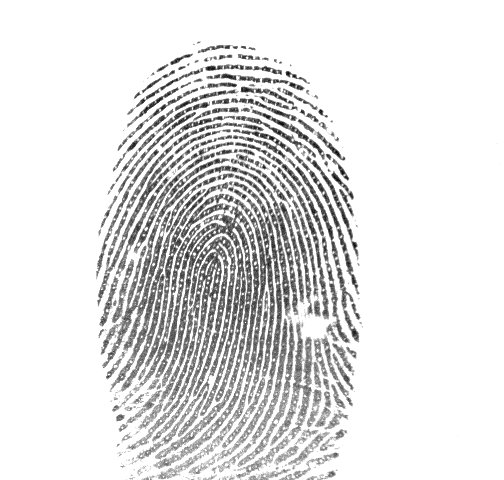
\includegraphics[width=0.3\columnwidth]{\figpath/fingerprint/input} &
%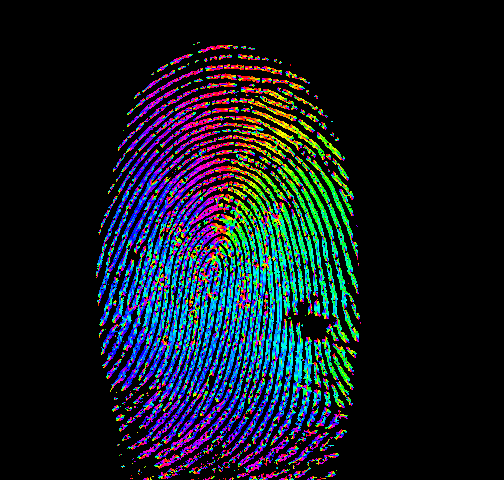
\includegraphics[height=0.15\textheight]{\figpath/fingerprint/ori_1st} &
%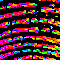
\includegraphics[height=0.15\textheight]{\figpath/fingerprint/ori_1st_zoom} \\
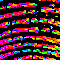
\includegraphics[width=0.3\columnwidth]{\figpath/fingerprint/ori_1st_zoom} &
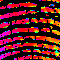
\includegraphics[width=0.3\columnwidth]{\figpath/fingerprint/ori_clover_zoom} \\
(a) & (b) & (c) \\
%&
%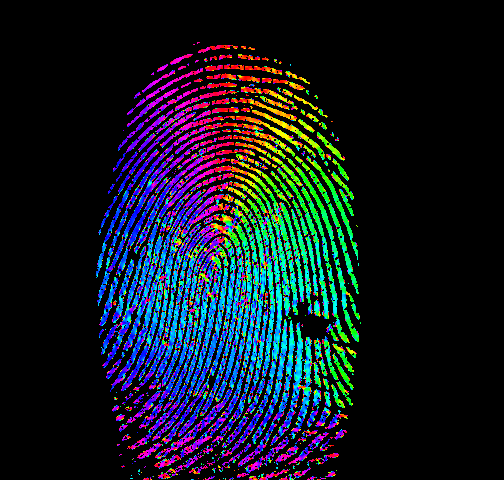
\includegraphics[height=0.15\textheight]{\figpath/fingerprint/ori_clover} &
%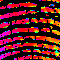
\includegraphics[height=0.15\textheight]{\figpath/fingerprint/ori_clover_zoom} \\
%		& (d) & (e)
\end{tabular}
%
\caption{Fingerprint images: %
(a) input image; %
(b,c) first derivative estimate of orientation with close-up; %
(d-e) second derivative estimate with close-up. Note the high errors at the centre of the ridge for first derivatives and at the edges of the ridge for second derivatives.}
\label{f:fingerprints}
\end{figure}
